\begin{figure}[htbp]
\centering
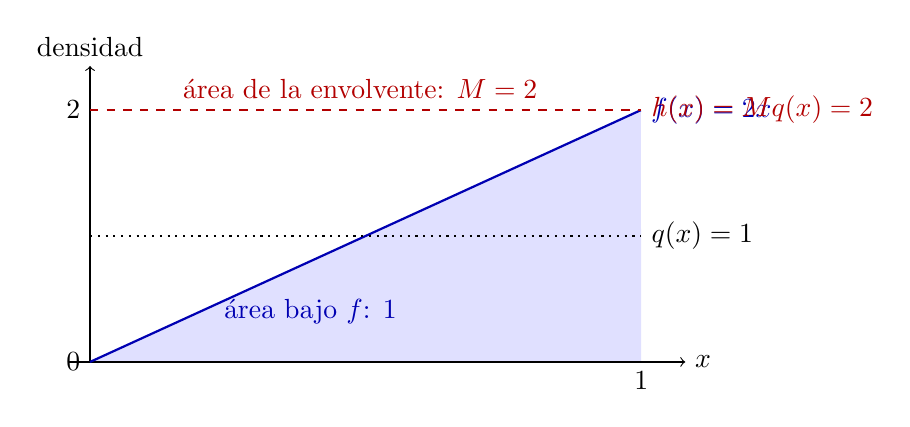
\begin{tikzpicture}[x=7cm,y=1.6cm]
  \fill[blue!12] (0,0) -- plot[domain=0:1,samples=60] (\x,{2*\x}) -- (1,0) -- cycle;
  \draw[->] (-0.04,0) -- (1.08,0) node[right] {$x$};
  \draw[->] (0,0) -- (0,2.35) node[above] {densidad};
  \draw[thick,blue!70!black,domain=0:1,samples=60] plot (\x,{2*\x})
    node[right] {$f(x)=2x$};
  \draw[thick,dashed,red!70!black] (0,2) -- (1,2)
    node[right] {$h(x)=Mq(x)=2$};
  \draw[thick,dotted] (0,1) -- (1,1)
    node[right] {$q(x)=1$};
  \draw (0,0) node[left] {$0$};
  \draw (0,2) node[left] {$2$};
  \draw (1,0) node[below] {$1$};
  \node[blue!70!black] at (0.40,0.40) {área bajo $f$: $1$};
  \node[red!70!black] at (0.49,2.17) {área de la envolvente: $M=2$};
\end{tikzpicture}
\caption{La densidad objetivo queda debajo de la envolvente. La propuesta es uniforme en $[0,1]$.}\label{fig:envolvente}
\end{figure}